\subsection{Hipótese 3}
\label{sec:resultados-hipotese-3}

Agora voltamos nossa atenção para a possível relação entre a aprendizagem e a satisfação, ritmo e relevância reportados pelos alunos.

\begin{figure}
	\centering

	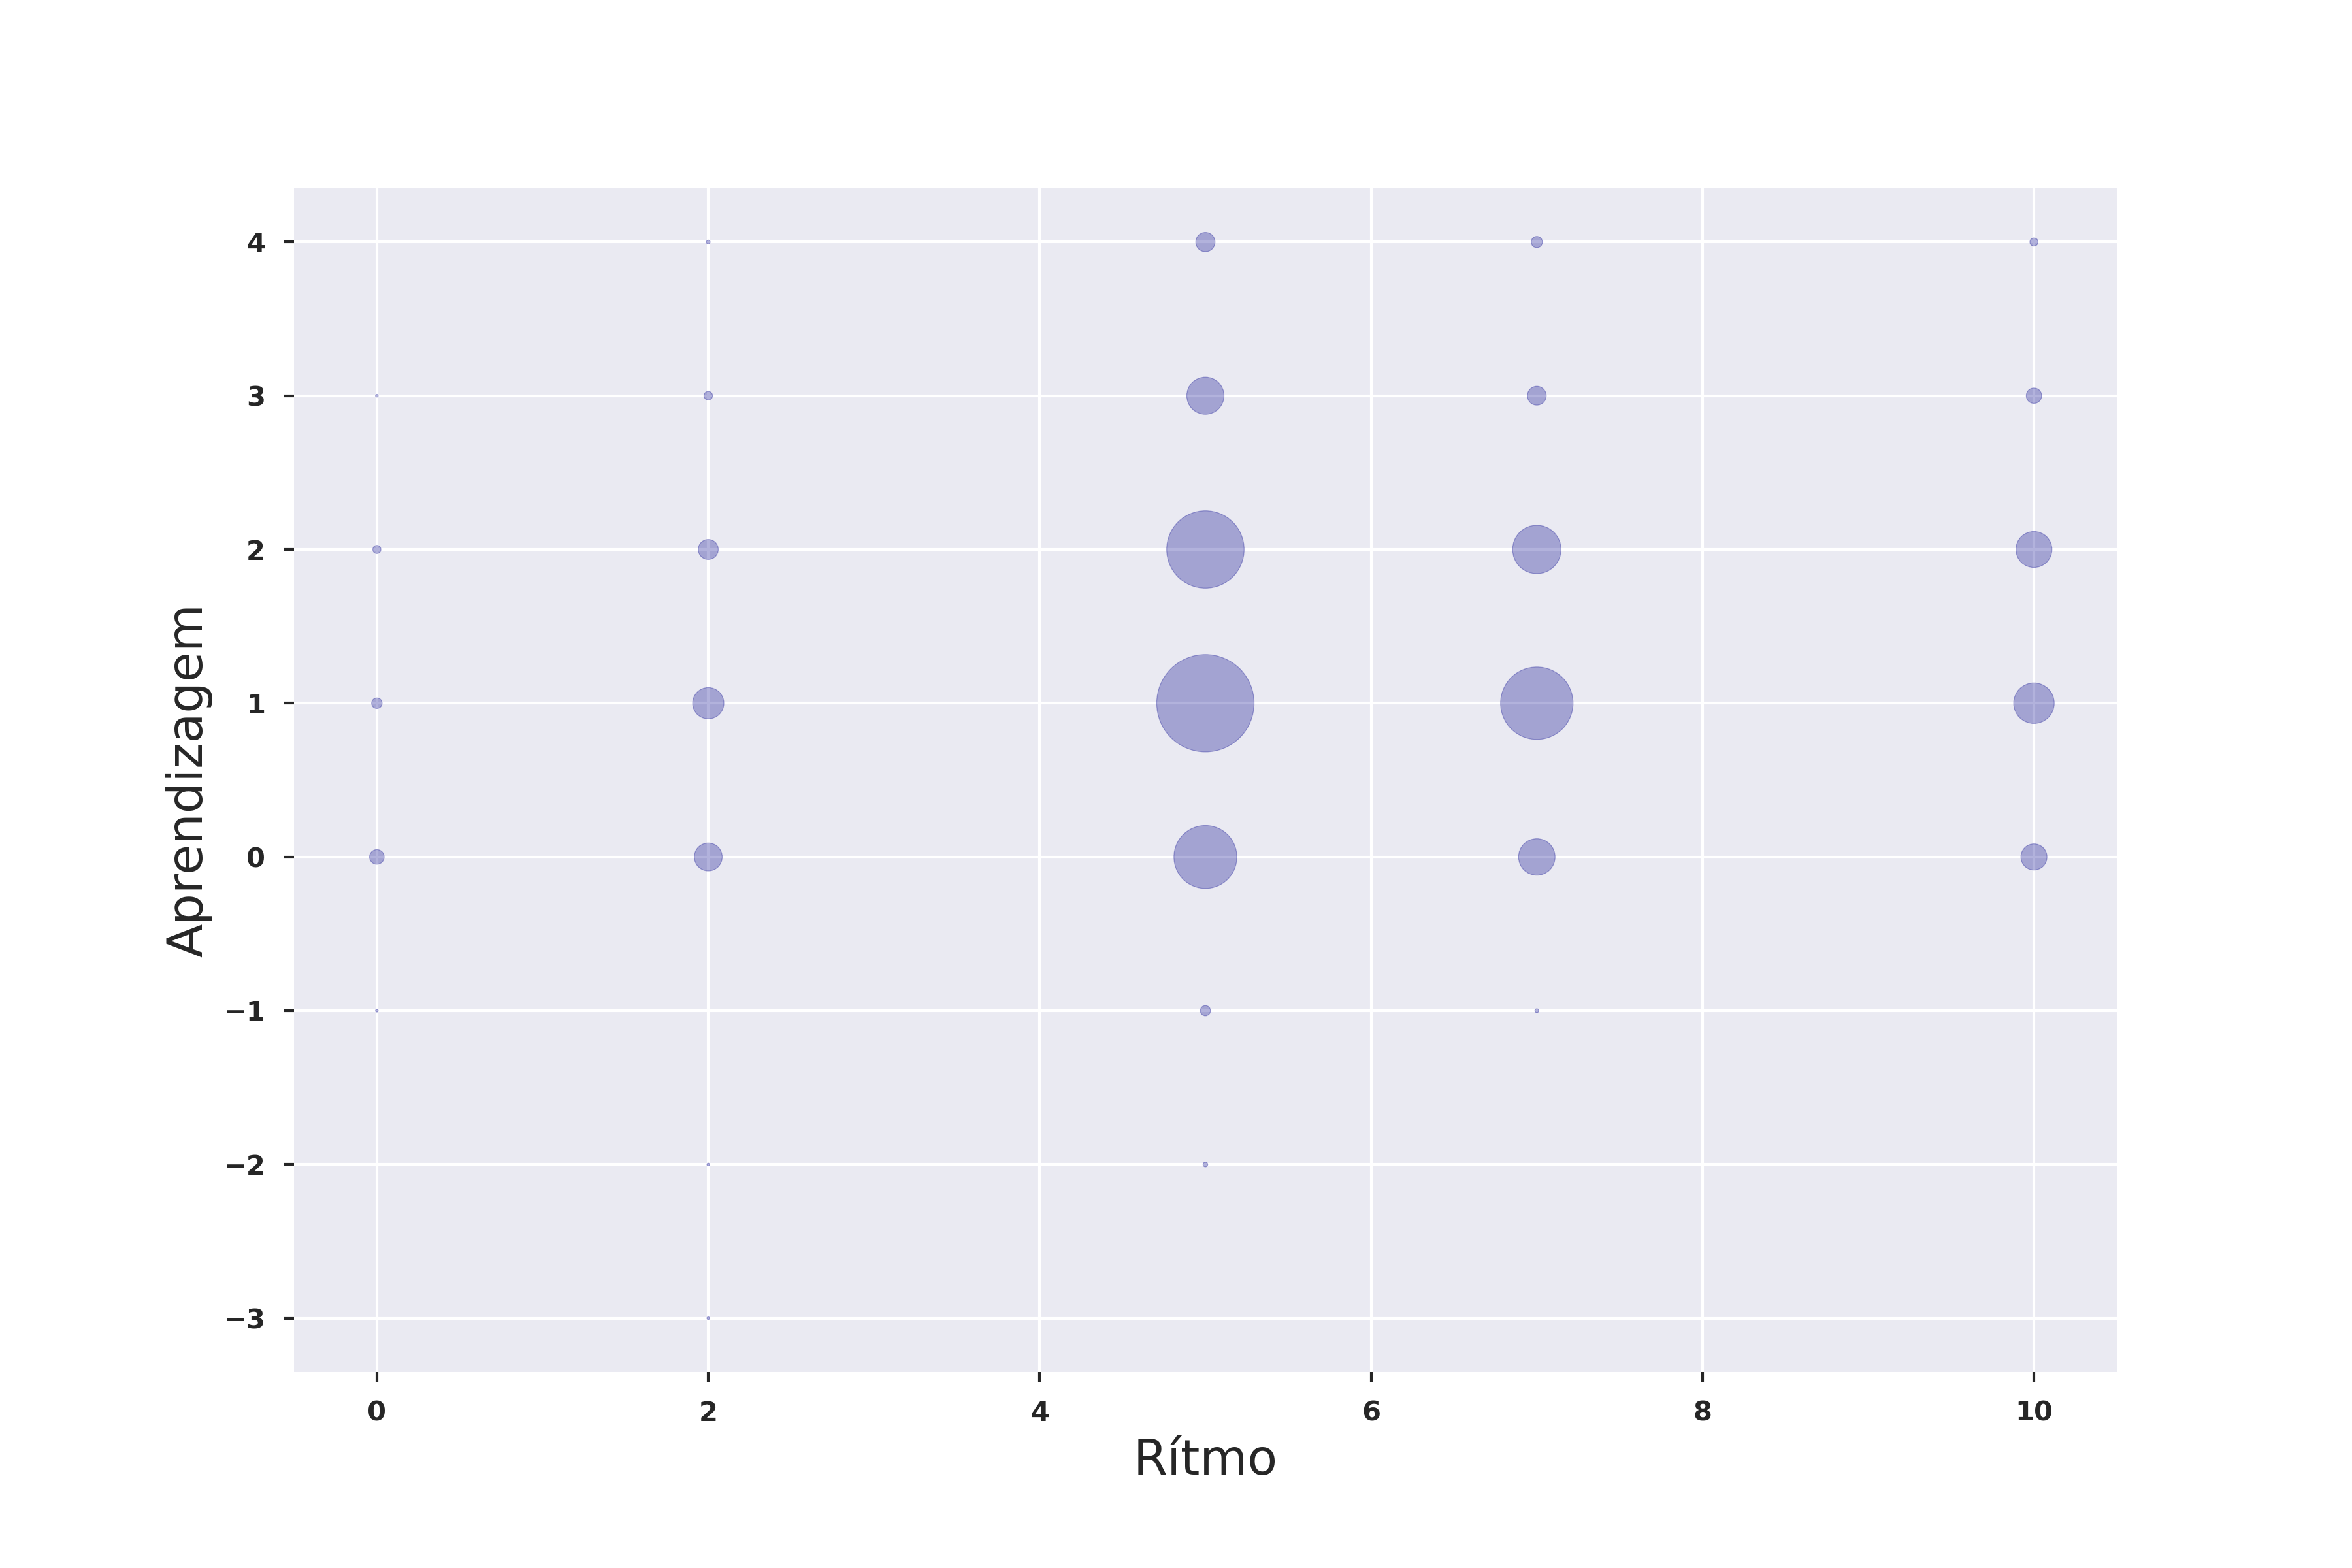
\includegraphics[width=0.33\textwidth]{aprendizagem-vs-ritmo}\hfill
	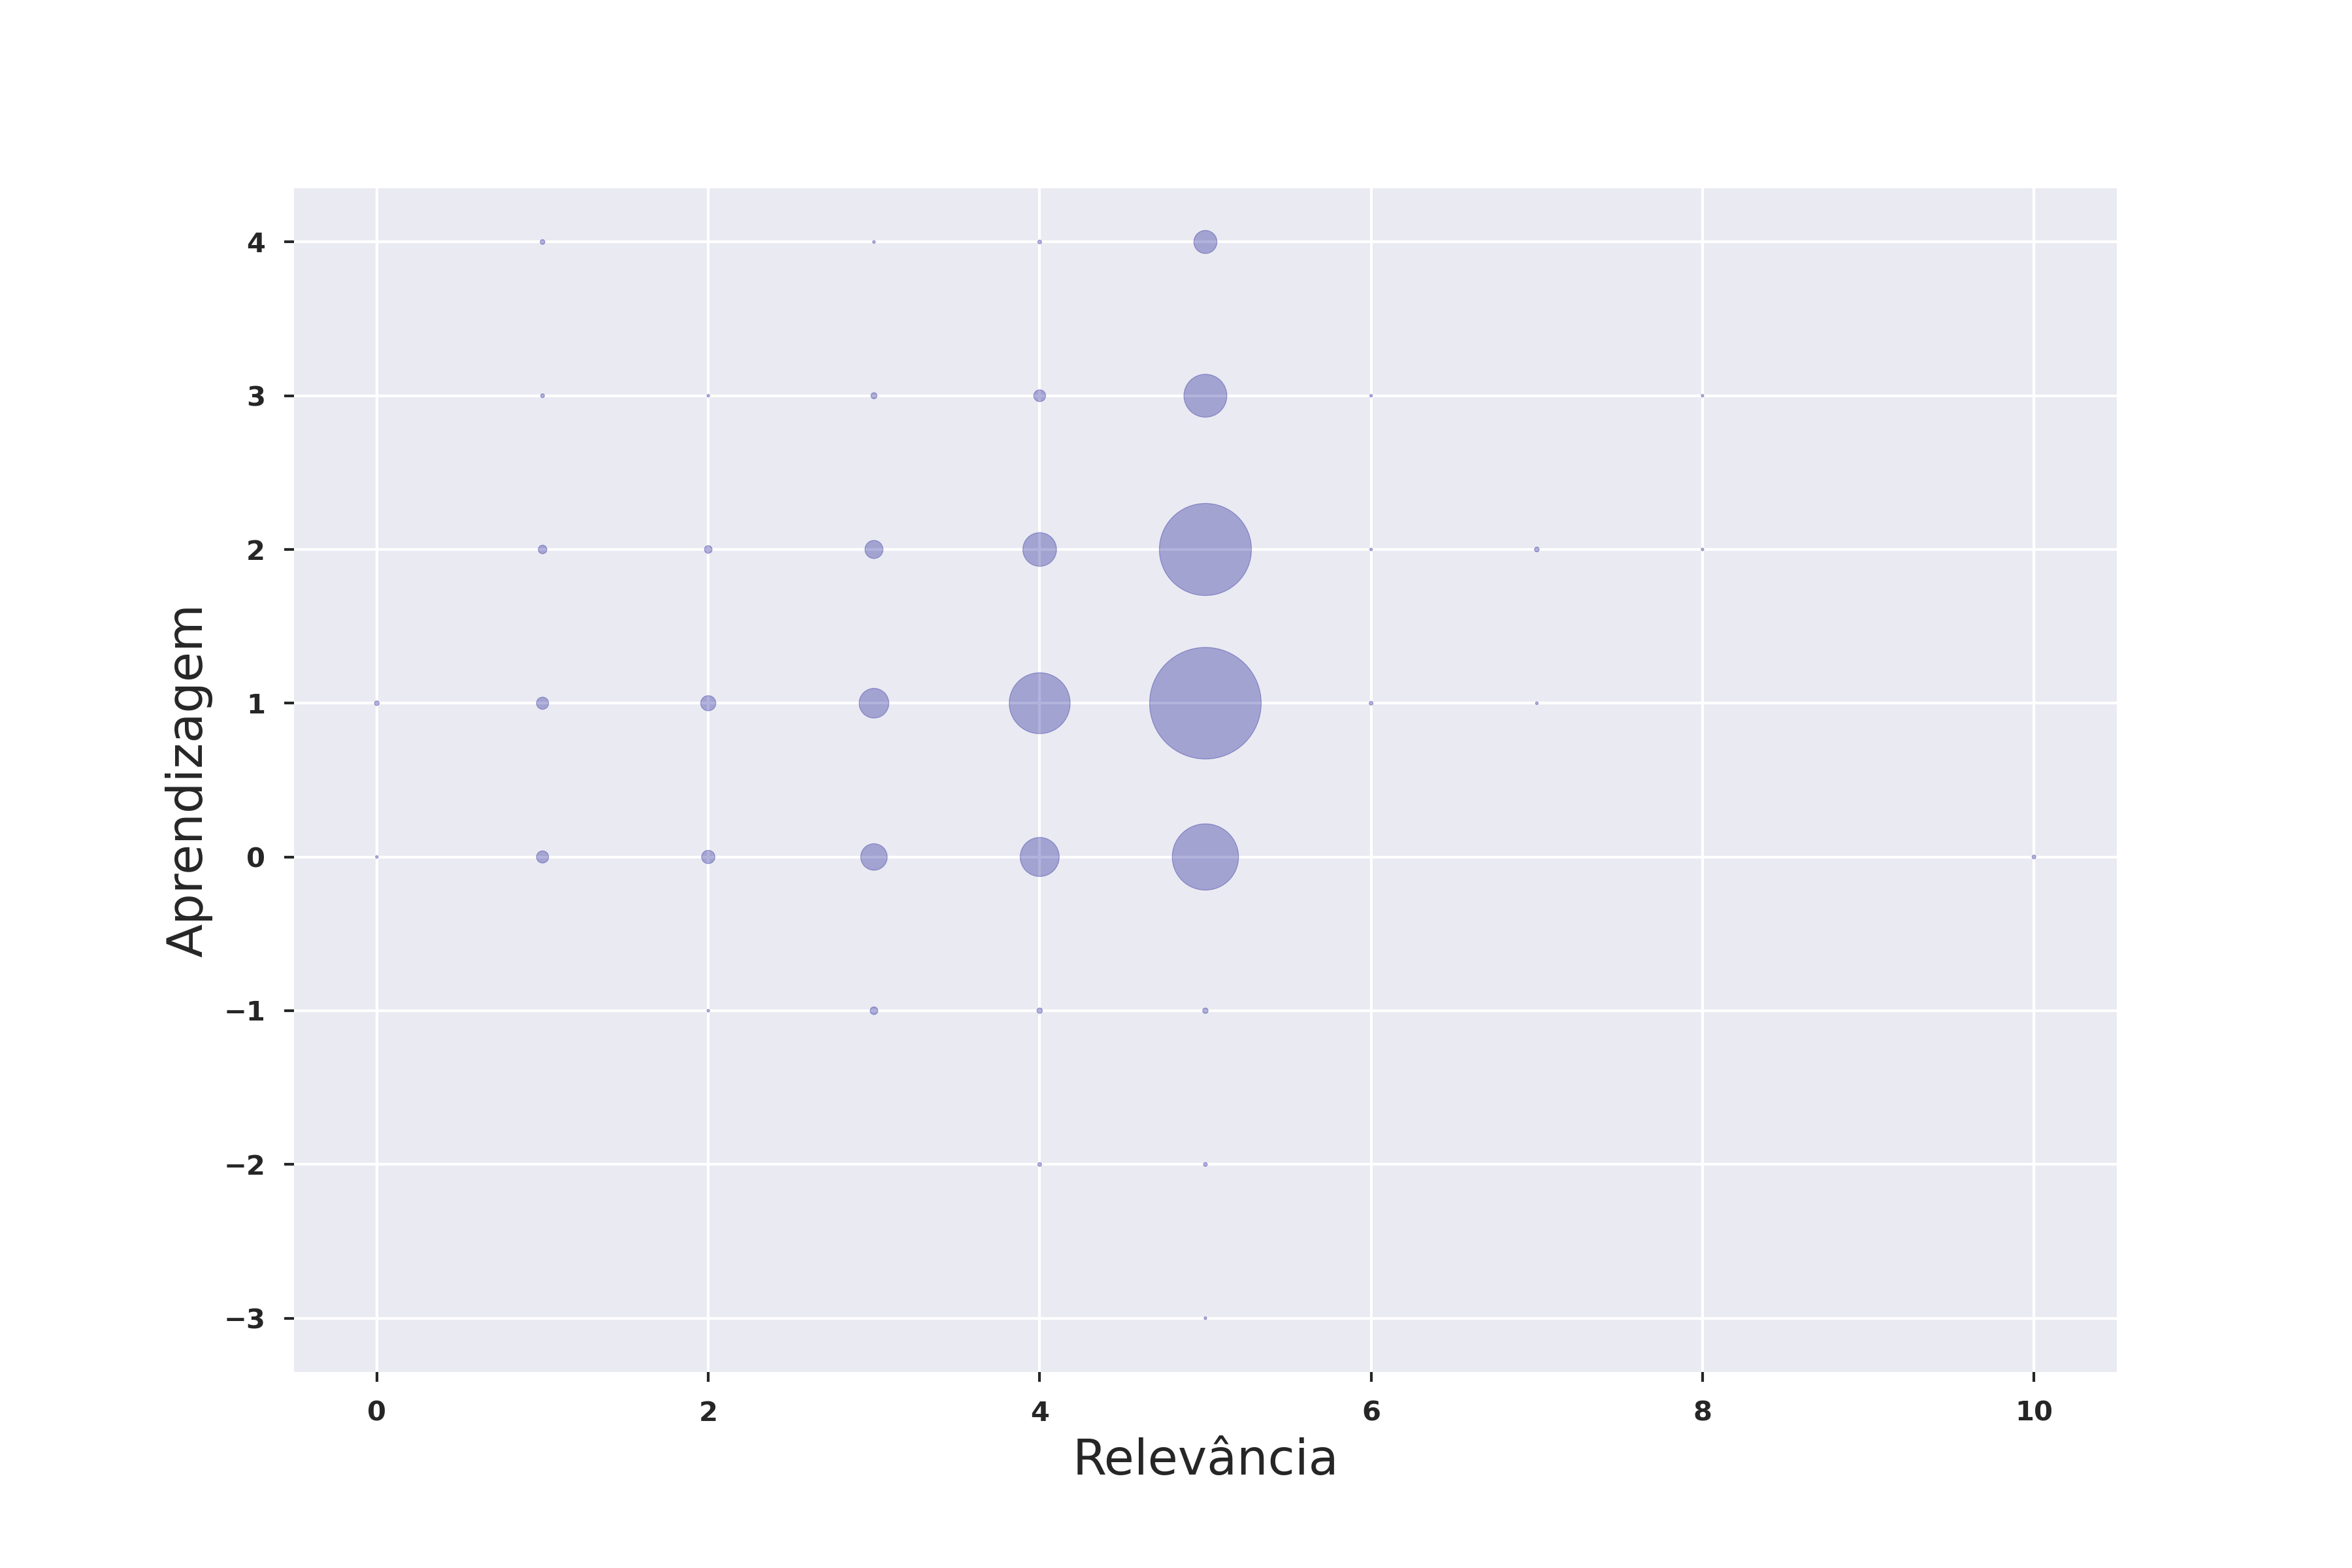
\includegraphics[width=0.33\textwidth]{aprendizagem-vs-relevancia}\hfill
	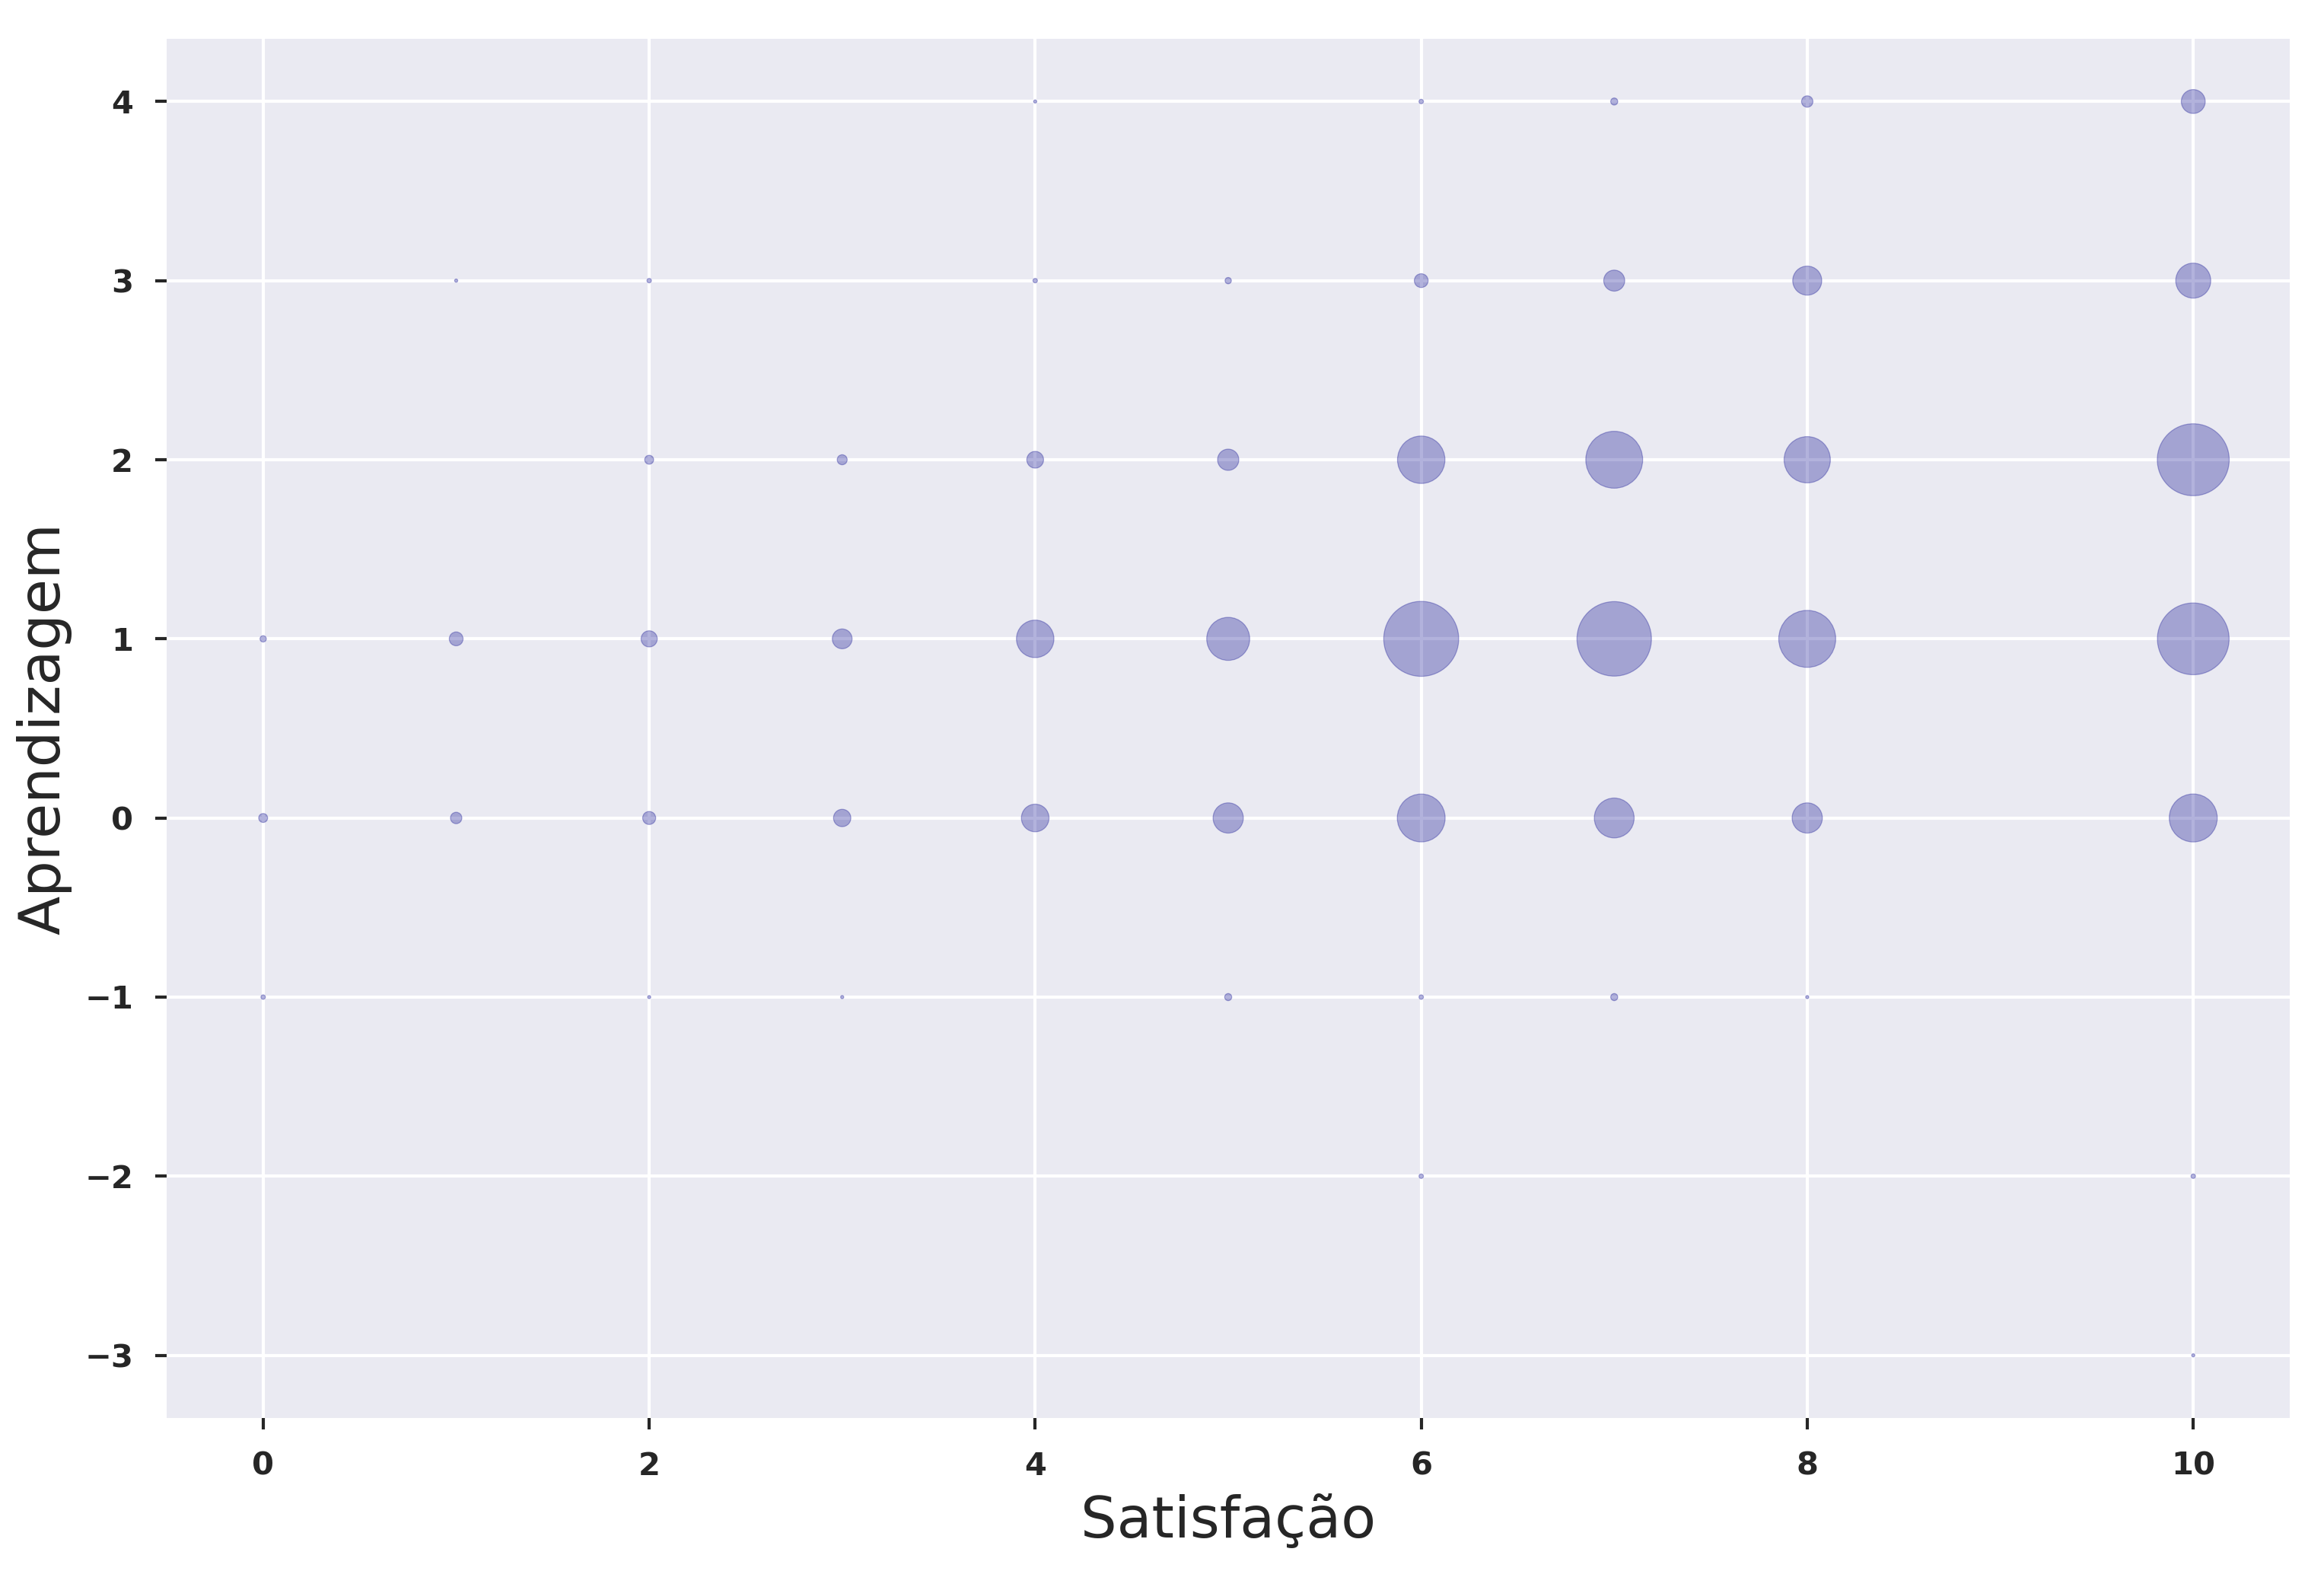
\includegraphics[width=0.33\textwidth]{aprendizagem-vs-satisfacao}%

	\caption{\foreign{Bubble-plot} da aprendizagem em função de cada um dos preditores.}
	\label{fig:bubble-plots}
\end{figure}

O argumento aqui é baseado na aprendizagem individualizada: o ritmo, que pode ser completamente controlado pelo aluno nessa abordagem, oferece vantagem para a aprendizagem.
E como temos informações extras sobre a satisfação e a relevância, vamos considerá-las também como critérios de comparação.

Como a aprendizagem $a$ é uma variável numérica, temos em mãos um problema de regressão.
Argumentamos que uma abordagem classificatória também é possível, desde que se tome o cuidado de garantir a integridade do espaço amostral de $a$, o intervalo $[-4,4]$.
Porém isso ficará para trabalhos futuros.

O modelo de regressão mais simples é o linear.
Porém, uma análise visual dos gráficos de aprendizagem em função de cada um dos preditores não torna evidente qualquer possível relação linear (fig.~\ref{fig:bubble-plots}).
Então experimentamos outros algoritmos de regressão, conforme apresentado na Tabela~\ref{tab:reg-ds-1}.

\begin{table}
	\centering
	\caption{Métricas de qualidade dos vários algoritmos de regressão aplicados a DS.}
	\label{tab:reg-ds-1}
	\begin{tabular}{llccc}
		\toprule
		Algoritmo   & Linear? &  RMSE &   MAE & $R^2$\\
		\midrule
		XGBoost  & Não     & 0,769 & 0,581 & \textbf{0,193}\\
		\foreign{Random Forest} & Não & 0,772 & 0,594 & 0,186\\
		Árvore de decisão & Não &  0,775 & 0,596 & 0,181\\
		Adaboost & Não     & 0,806 & 0,629 & 0,113\\
		\foreign{ElasticNet} & Sim & 0,819 & 0,640 & 0,083\\
		SVR & Não & 0,835 & 0,612 & 0,048\\
		\bottomrule
	\end{tabular}
\end{table}

\begin{table}
	\centering
	\caption{$R^2$ e $\bar R^2$ para o algoritmo XGBoost aplicado a DA e DS.}
	\label{tab:r2-adjusted}
	\begin{tabular}{ccccccc}
		\toprule
		           &            &            & \multicolumn{2}{c}{ Data Science  } & \multicolumn{2}{c}{ Data Analytics }\\
		\midrule
		Relevância & Ritmo      & Satisfação & $R^2$     & $\bar R^2$ & $R^2$     & $\bar R^2$\\
		\midrule
		\checkmark & \checkmark & \checkmark & 0,193 & 0,191 & 0,213 & 0,211 \\
		           & \checkmark & \checkmark & 0,125 & 0,120 & 0,184 & 0,183 \\
		\checkmark &            & \checkmark & 0,115 & 0,114 & 0,147 & 0,146 \\
		           &            & \checkmark & 0,075 & 0,074 & 0,130 & 0,130 \\
		\checkmark & \checkmark &            & 0,071 & 0,070 & 0,096 & 0,095 \\
		\checkmark &            &            & 0,052 & 0,051 & 0,019 & 0,018 \\
		           & \checkmark &            & 0,014 & 0,014 & 0,076 & 0,075 \\
		\bottomrule
	\end{tabular}
\end{table}

\begin{table}[b]
	\centering
	\caption{Métricas de desempenho dos vários algoritmos de regressão aplicados a DA.}
	\label{tab:reg-da-1}
	\begin{tabular}{llccc}
		\toprule
		Algoritmo               & Linear? & RMSE  &   MAE & $R^2$\\
		\midrule
		XGBoost                 & Não     & 0,958 & 0,760 & \textbf{0,213}\\
		Árvore de decisão       & Não     & 0,958 & 0,762 & 0,212\\
		\foreign{Random Forest} & Não     & 0,959 & 0,770 & 0,210\\
		Adaboost                & Não     & 0,983 & 0,801 & 0,170\\
		\foreign{ElasticNet}    & Sim     & 0,985 & 0,793 & 0,167\\
		SVR                     & Não     & 0,994 & 0,797 & 0,152\\
		\bottomrule
	\end{tabular}
\end{table}

O conjunto de dados usado para as regressões foi extraído do conjunto completo (Figura~\ref{fig:dataset}), tomando o cuidado de que um dado aluno não estivesse presente mais do que uma vez.
Fizemos esse tratamento com o intuito de evitar correlação entre os exemplos.

Em seguida, aplicamos cada um dos algoritmos a 70\% dos exemplos no conjunto de dados (conjunto de treinamento), explorando sistematicamente o espaço de hiper-parâmetros à procura de um mínimo global no erro quadrático médio da regressão.

O melhor índice de determinação, calculado sobre os 30\% exemplos restantes (conjunto de teste), foi $R^2 \approx 0,193$ para o modelo XGBoost, composto por um conjunto de árvores de decisão simples \cite{Friedman2001}.
Isso significa que nosso melhor modelo é capaz de explicar apenas 19\% das variações na aprendizagem, a partir dos preditores propostos.
Embora seja baixo, podemos argumentar  que a aprendizagem sofre maior influência de outros parâmetros mais importantes, que não temos acesso aqui, como a metodologia de aprendizagem, a qualidade das atividades e conteúdo proposto \etc.



Agora que sabemos que o modelo XGBoost obteve melhor desempenho, podemos experimentar variar os preditores: efetuamos a regressão considerando como preditores as combinações de um, dois e três preditores.
Nesse caso, a métrica mais relevante é o $\bar R^2$, que pondera o índice de determinação pela quantidade de preditores.
Por exemplo, para dois modelos com o mesmo $R^2$, o primeiro com um e o segundo com dois preditores, o melhor modelo é aquele com maior $\bar R^2$.

Os resultados desse experimento estão na Tabela~\ref{tab:r2-adjusted}, ordenados por $R^2$ e $\bar R^2$.
Concluimos que o melhor modelo é de fato o que utiliza todos os três preditores propostos: satisfação, relevância e ritmo.



A mesma análise pode ser feita para DA, o que nos leva inicialmente à escolha do algoritmo, conforme ilustra a Tabela~\ref{tab:reg-da-1}.
Curiosamente, nesse caso o algoritmo de árvore de decisão obteve melhor desempenho que o \foreign{random forest} (o oposto para DS).
Ainda assim, novamente o melhor (maior $R^2$) algoritmo foi o XGBoost; porém com $R^2$ similar ao caso de DS.

Em seguida variamos os preditores e obtemos os resultados apresentados na Tabela~\ref{tab:r2-adjusted}.
O resultado é similar ao de DS: o modelo que utiliza todos os preditores é melhor.



Resumindo, para DA e DS o melhor modelo XGBoost utilizando os três preditores propostos consegue explicar apenas aproximadamente 20\% das variações observadas (hipótese 3).
Ainda assim, o fato de $R^2$ ser demasiadamente baixo torna essa conclusão duvidosa.
